\documentclass[conference]{IEEEtran}
\IEEEoverridecommandlockouts
% The preceding line is only needed to identify funding in the first footnote. If that is unneeded, please comment it out.
\usepackage{cite}
\usepackage{amsmath, amssymb, amsfonts}
\usepackage{algorithmic}
\usepackage{graphicx}
\usepackage{textcomp}
\usepackage{fourier}
%\usepackage{libertinust1math} % - cool one
\usepackage{MnSymbol}
\usepackage[english]{babel}
\usepackage[fixlanguage]{babelbib}
\usepackage[unicode=true,hidelinks]{hyperref}

\begin{document}

\renewcommand*{\figureautorefname}{Fig.}
\renewcommand*{\equationautorefname}{Eq.}

\def \w{\omega}

% ------------------------- %

\def \eq{\begin{equation}}
\def \qe{\end{equation}}
\def \eqc{\begin{equation*}}
\def \cqe{\end{equation*}}

% ------------------------- %
% ------------------------- %

\newcommand{\shifthat}[2]{%
    \stackengine{\Sstackgap}{$#2$}{\(\hspace{#1}\hat{}\)}{O}{l}{F}{T}{S}
}

% ------------------------- %

\newcommand{\operator}[2][operator]{
    \if H#2\shifthat{0.5em}{#2}\else
    \if d#2\shifthat{0.49em}{#2}\else
    \if q#2\shifthat{0.35em}{#2}\else
    \if \mu#2\shifthat{0.35em}{#2}\else
    \shifthat{0.45em}{#2}
    \fi
    \fi
    \fi
    \fi
}

% ------------------------- %

\newcommand{\vectoperator}[2][operator]{
    \if d#2\shifthat{0.367em}{\textbf{#2}}\else
    \if m#2\shifthat{0.4em}{\textbf{#2}}\else
    \shifthat{0.275em}{\textbf{#2}}
    \fi
    \fi
}

% ------------------------- %

\newcommand{\vect}[3][vector]{
    \overrightarrow{#2_{#3}}
}

% ------------------------- %

\newcommand{\vectbf}[2][bold vector]{
    \vect{\textbf{#2}}
}

% ------------------------- %

\newcommand{\pd}[3][empty]{
    \frac{\partial {#2}}{\partial {#3}}
}

% ------------------------- %

\newcommand{\func}[5][empty]{
    {#2}_{#3}^{#4} \left({#5} \right)
}

% ------------------------- %

\newcommand{\underrel}[3][]{
    \mathrel{\mathop{#3}\limits_{
        \ifx c#1\relax\mathclap{#2}\else#2\fi
    }}
}
% ------------------------- %

\makeatletter

\newcommand{\Autoref}[1]{\@first@ref#1,@}
\def\@throw@dot#1.#2@{#1}% discard everything after the dot
\def\@set@refname#1{%    % set \@refname to autoefname+s using \getrefbykeydefault
    \edef\@tmp{\getrefbykeydefault{#1}{anchor}{}}%
    \xdef\@tmp{\expandafter\@throw@dot\@tmp.@}%
    \ltx@IfUndefined{\@tmp autorefnameplural}%
        {\def\@refname{\@nameuse{\@tmp autorefname}}}%
        {\def\@refname{\@nameuse{\@tmp autorefnameplural}}}%
}
\def\@first@ref#1,#2{%
\ifx#2@\autoref{#1}\let\@nextref\@gobble% only one ref, revert to normal \autoref
\else%
    \@set@refname{#1}%  set \@refname to autoref name
    \@refname\ref{#1}% add autoefname and first reference
    \let\@nextref\@next@ref% push processing to \@next@ref
\fi%
\@nextref#2%
}
\def\@next@ref#1,#2{%
\ifx#2@,~\ref{#1}\let\@nextref\@gobble% at end: print and+\ref and stop
\else, \ref{#1}% print  ,+\ref and continue
\fi%
\@nextref#2%
}

\makeatother

% ------------------------- %
% ------------------------- %

\newcommand{\img}[4][anything]{
    \begin{figure}[H]{
        \center{\includegraphics[width={#4}]{{#1}}}
        \caption{#2}\label{#3}}
    \end{figure}
}

% ------------------------- %

\newcommand{\floatimg}[4][anything]{
    \begin{figure}[ht]{
        \center{\includegraphics[width={#4}]{{#1}}}
        \caption{#2}\label{#3}}
    \end{figure}
}

% ------------------------- %

\newcommand{\subimg}[2][anything]{
    \begin{minipage}[h]{{#2}} % 0.4\textwidth
        \center{\includegraphics[width=1\linewidth]{{#1}}}
    \end{minipage}
}

% ------------------------- %

\newcommand{\subimgtwo}[4][anything]{
    \subfloat[{#2}]{\includegraphics[width={#4}]{{#1}}\label{#3}}
}

% ------------------------- %

\title{Angular dispersion boost of high order laser harmonics with dense
plasma clusters}
% {\footnotesize \textsuperscript{*}\textit{Note: Sub-titles are not captured in Xplore and
% should not be used (this footnote should be deleted)}}
% \thanks{Identify applicable funding agency here. If none, delete this.}
% }

\author{
	\IEEEauthorblockN{L.A. Litvinov\textsuperscript{1}, A.A. Andreev\textsuperscript{1, 2}}
	\IEEEauthorblockA{\textsuperscript{1}Saint Petersburg State University, Saint Petersburg, Russia}
	\IEEEauthorblockA{\textsuperscript{2}Ioffe Physico-Technical Institute, Saint Petersburg, Russia}
}


\maketitle

\begin{abstract}
	Periodic surface gratings or photonic crystals are excellent tools for diffracting light and to collect
	information about the spectral intensity, if the target structure is known, or about the diffracting
	object, if the light source is well defined. However, this method is less effective in the case of extreme
	ultraviolet (XUV) light due to the high absorption coefficient of any material in this frequency range.
	Here we propose a nanosphere array target in the plasma phase as an efficient dispersive medium for
	the intense XUV light which is originated from laser-plasma interactions where various high harmonic
	generation processes take place. The scattering process is studied with the help of numerical
	simulations and we show that the angular distribution of different harmonics after scattering can be
	perfectly described by a simple interference theory.
\end{abstract}

% \begin{IEEEkeywords}
% component, formatting, style, styling, insert
% \end{IEEEkeywords}

\section{Introduction}

Limited size targets interacting with high-intensity coherent radiation is well-studied phenomenon of linear excited surface plasmonic oscillations. Absorption and scattering of incident light in this case good described with Mie theory predicting exist of resonance corresponding to multipole oscillations of part of the target free electrons relative to positive charged ions. In resonance mode efficient exciting of surface plasmons can lead to significant boost internal and external field on fundamental cluster frequency (eigenfrequency). In turn, this can cause enhancement of field scattered on large angles relative to the direction of incident wave.

In micrometer wavelengths photon crystals and lattices can be used for direction or diffraction electromagnetic waves~\cite{lin_zhang}, while for x-ray radiation it is possible to use real crystals with regularly placed scattering centers (atoms) with distance of few nanometers~\cite{batterman_cole}. At the same time, large interval between these wavelength orders named XUV (extreme-ultraviolet) is hard to manipulate.

Within the present work we consider the possibility of directed scattering of short wavelength radiation in the XUV range by scattering on suitable spherical clusters. Similar case with cylindrical symmetry (arrays of nanocylinders as scatters) was researched earlier~\cite{andreev_lecz}. Of course, nanocylinders are more suitable regarding the control of size an distance parameters at the target manufacturing stage, but arrays of spherical clusters can make possible to manipulate with light direction in three-dimensional space and give a more optimal spatial configuration.

\section{Base model}

\subsection{Dielectric function}

Firstly we consider a single cluster with radius $a$ irradiated by short femtosecond pulse with intensity about $I_{h} \approx 10^{14}$ $\textrm{W/cm}^2$. The Drude model yields the dielectric function of the plasma:

	\eq
		\varepsilon (\w) = 1 - \left( \frac{\w_{pe}}{\w} \right)^2 \frac{1}{1 + i \beta_{e}}, \qquad \w_{pe} = \sqrt{\frac{4 \pi e^2 n_e}{m_e}},
		\label{eps_plasma}
	\qe

\noindent where $\w$ --- harmonic (angular) frequency under consideration; $\w_{pe}$ --- the electron plasma frequency; $e$, $m_e$ --- electron charge and mass; $n_e = Z n_i$ --- the electron number density, where $Z$ --- average ionization degree, $n_i$ --- ion density. $\beta_{e} = v_e / \w$ and $v_e$ --- electron-ion collision rate in Spitzer approximation. As we are going to consider scattering of harmonic radiation, the cluster should have a density above the critical one for this harmonic: $n_c = \w^2 m_e / 4 \pi e^2$. For 10-th Ti:Sa laser harmonic with wavelength $\lambda_{L} = 830$ nm one obtains condition $n_e > 1.3 \cdot 10^{23}$ $\textrm{cm}^{-3}$.

\subsection{Mie Theory}

In the case of linear interaction Mie theory can be used for the description of elastic electromagnetic waves scattering by arbitrary sized particles and beyond that, it allows the description of the electric and magnetic field distribution inside and outside the scatter \cite{boren_huffman}. A main step is to solve the scalar Helmholtz Equation in suitable coordinate system and gain the vector solutions. For spherical cluster the solution of corresponding equation can be written in a spherical Bessel function of the $l$-th kind and $n$-th order the spherical harmonic including the associated Legendre polynomial~\cite{boren_huffman}.

Assume an incident plane wave propagating along $z$ axis of cartesian coordinate system and polarized along $x$ axis:

    \eq
        \vectbf{E}{i} = E_0\:e^{i\w t - ikz}\:\vectbf{e}{x},
        \label{E_i_sph}
    \qe

\noindent where $k = \w/c$ --- wavenumber, $\vectbf{e}{x}$ --- the unit vector of $x$ axis direction and polarization vector.

Now we can expand the plane wave into series using generalized Fourier expantions. Assuming our media is isotropic we obtain following form of scattered field~\cite{boren_huffman}:

    \eq
		\vectbf{E}{s} = \sum_{n = 1}^{\infty}E_n \left[ i a_n\left(ka, m\right) \vectbf{N}{}^{(3)}_{e1n} - b_n\left(ka, m\right) \vectbf{M}{}^{(3)}_{o1n} \right]
        \label{E_s_sph}
	\qe
	\eqc
		E_n = i^{n} E_0 \frac{2n + 1}{n \left(n + 1\right)}
	\cqe

$n$ --- vector harmonic number after cartesian-spherical coordinate system transformation, $m = \sqrt{\varepsilon\left(\w\right)}$ --- refractive index of the target.

Coefficients in \autoref{E_s_sph} have the following form~\cite{boren_huffman}:

    \eq
		a_n(x,\:m) = \frac{m \func{\psi}{n}{\prime}{x} \func{\psi}{n}{}{mx} - \func{\psi}{n}{\prime}{mx} \func{\psi}{n}{}{x}}{m \func{\xi}{n}{\prime}{x} \func{\psi}{n}{}{mx} - \func{\psi}{n}{\prime}{mx} \func{\xi}{n}{}{x}},
		\label{an_bessel}
	\qe

    \eq
        b_n(x,\:m) = \frac{\func{\psi}{n}{\prime}{x} \func{\psi}{n}{}{mx} - m \func{\psi}{n}{\prime}{mx} \func{\psi}{n}{}{x}}{\func{\xi}{n}{\prime}{x} \func{\psi}{n}{}{mx} - m \func{\psi}{n}{\prime}{mx} \func{\xi}{n}{}{x}},
        \label{bn_bessel}
    \qe
	\eqc % artificial indent after the equation
    \cqe %

\noindent where $\func{\psi}{n}{}{z} = z \func{j}{n}{}{z}$, $\func{\xi}{n}{}{z} = z \func{h}{n}{}{z}$ --- Riccati-Bessel functions, $h_n = j_n + i \gamma_n$ --- spherical Hankel functions of the first kind.

\subsection{Resonance conditions}

To investigate the conditions under which resonant field enhancement occur the determination of the desired coefficients (\Autoref{an_bessel, bn_bessel}) is necessary in general. Since we are only interested in particle sizes which are smaller than the incident wavelength we use the limiting forms of the respective Bessel functions. In this asymptotic limit the coefficients are of a much simpler form:

	\eq
		a_n\left( x \to 0,\:m \right) = \left( 1 + i C_n \frac{\left(m^2 + \frac{n + 1}{n} \right)}{(m^2 - 1)} \frac{1}{x^{2n+1}} \right)^{-1},
	\label{ab_asymp}
	\qe
	\eqc
		b_n\left( x \to 0,\:m \right) = 0,
	\cqe
	\eqc
		C_n = \frac{1}{2^{2n - 1}}\frac{ (2n - 1)! (2n + 1)!}{n! (n + 1)!}
	\cqe
	\eqc
	\cqe

In this case amplitude of the scattered field is maximum for $m^2 = - (n+ 1) / n$ when $ka \ll 1$, that gain corresponding set of resonance densities in collision-less case:

	\eqc
		n_e = \frac{2n + 1}{n}n_c.
	\cqe

\autoref{ab_asymp} can be used instead of \Autoref{an_bessel, bn_bessel} for scatters with quite small radius, but for $ka \sim 1$ the approximation ceases to be reasonable already, particularly for large $n$. In this case the first-order approximation, that can be obtained including first term in polynomial expansion of Bessel functions, is better suited \cite{abra_steg}. Moreover, in first-order approximation dependency of coefficients on the scatter size occurs, which lead to corresponding dependency of resonance electron density (\autoref{nenc_123:image}).

	\begin{figure}[htbp]
		\centerline{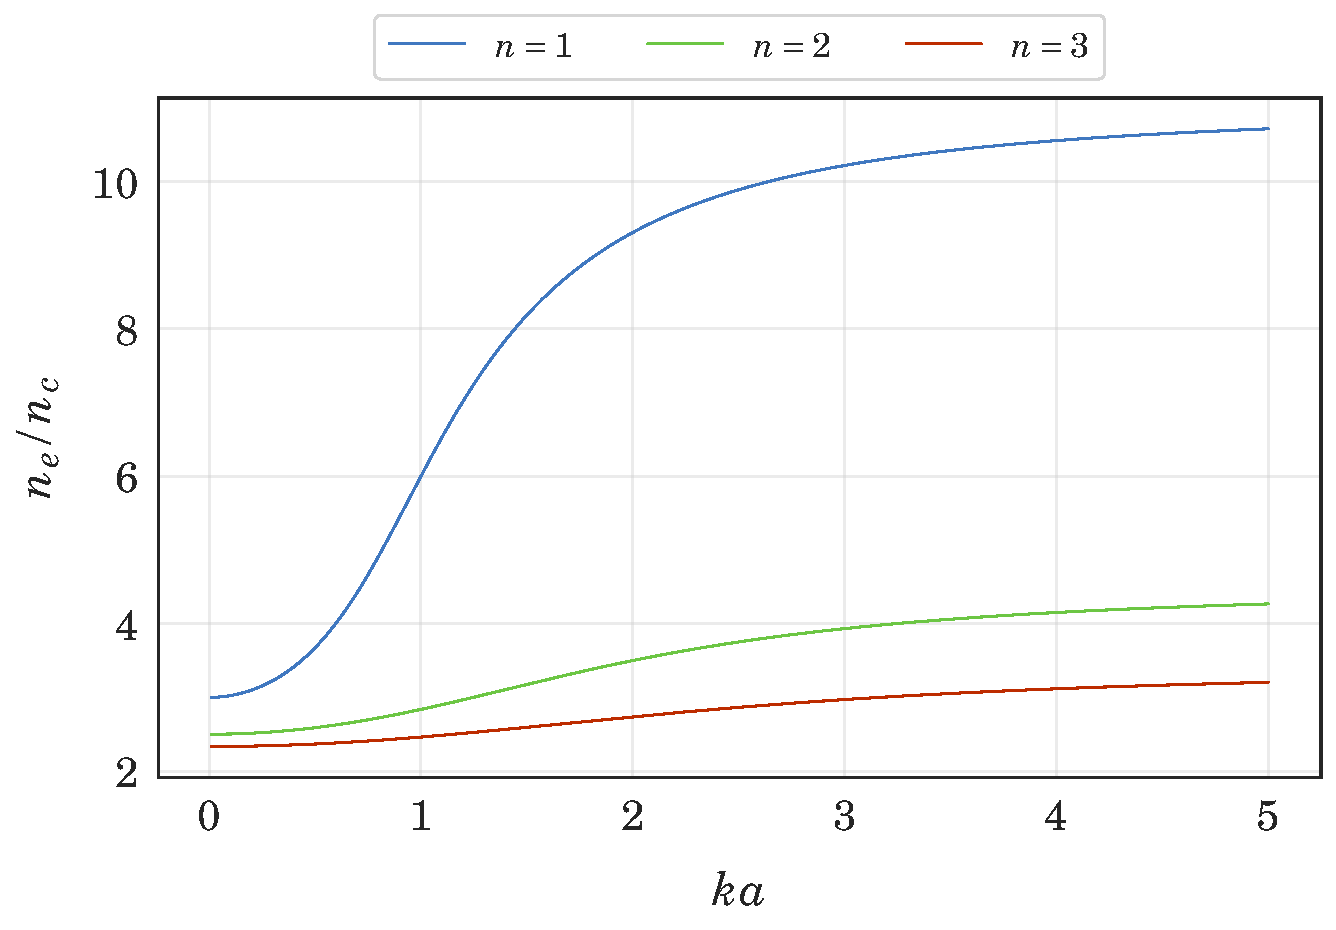
\includegraphics[width=\columnwidth]{../components/img/sph_base/nenc_123.pdf}}
		\caption{Resonance electron density depending on radius in collision-less case.}
		\label{nenc_123:image}
	\end{figure}

Such approximations allow us to estimate the resonance cases for a material with pre-defined refractive index $m$ as well as estimate refractive index corresponding to the required wavelength. As we consider XUV range radiation (20-120 nm), radiuses of spherical scatters should be about few nanometers, that causes $ka \sim 1$. Obviously, for such $ ka $ the resonance values of the electron density can be large in considering $n = 1$ as term with the largest contribution to the scattered field. Staying within high-temperature plasma we should use only $n_e < 10^{24}$ $\textrm{cm}^{-3}$.

In first-order approximation with wavelength $\lambda_{10} = \lambda_{L} / 10 = 83$ nm, we have $n_e \approx 5.7 \cdot 10^{23}$ $\textrm{cm}^{-3}$ for $ka = 0.7$ ($a \approx 8.91$ nm) to reach efficient scattering.

\section{Simulations}

\subsection{Scattering by a single cluster}

\subsection{Scattering by an array}

Using resonance conditions obtained with analytical model, we consider diffraction by arrays of plasma clusters. Simple cubic lattice with $N = 12$ edge nodes and different grating constant $d$ is considered spatial configuration of a volume grating. As the incident field we use gaussian beam with width $w = 300$ nm, that allow to assume the lattice as cluster layers by continuing cubic structure periodically along the entrance surface vector.

Diffraction orders can be obtained with Bragg's law \cite{kress_bernard}:

	\eq
		2d \sin(\theta + \varphi) = n\lambda
		\label{bragg_wulfe}
	\qe

\noindent where $d$ --- the fringe spacing of the grating, $\theta$ --- the angle between the incident beam and the normal to the entrance surface, $\phi$ --- the angle between the normal and the grating vector, $n$ --- the order of diffraction, $\lambda$ --- diffracted wavelength. As we choose cubic lattice, $\varphi = 0$ due to the symmetry, that lead to planar Wolfe–Bragg's condition.

According to \autoref{bragg_wulfe} we obtain $\theta = \arcsin\frac{1}{4}$ for grating with $d = 2\lambda$ and $\theta = \arcsin\frac{1}{6}$ for grating with $d = 3\lambda$ in $1$-st diffraction order. Using these values we numerically compute the scattered field of 10-th laser harmonic with wavelength $\lambda_{10} = 83$ nm, using CELES package, based on T-matrix calculations~\cite{t_matrix, celes}.

We can see directions corresponding to the angular boost of the incident beam, in particular, for $d = 2\lambda_{10}$ there are two fairly clear directions (\autoref{14.324deg:image}), while for $d = 3\lambda_{10}$ there are three less clear ones with wider spread of the scattered field in general (\autoref{9.594deg:image}).

% \subsection{Abbreviations and Acronyms}\label{AA}
% Define abbreviations and acronyms the first time they are used in the text, 
% even after they have been defined in the abstract. Abbreviations such as 
% IEEE, SI, MKS, CGS, ac, dc, and rms do not have to be defined. Do not use 
% abbreviations in the title or heads unless they are unavoidable.

% \subsection{Units}
% \begin{itemize}
% \item Use either SI (MKS) or CGS as primary units. (SI units are encouraged.) English units may be used as secondary units (in parentheses). An exception would be the use of English units as identifiers in trade, such as ``3.5-inch disk drive''.
% \item Avoid combining SI and CGS units, such as current in amperes and magnetic field in oersteds. This often leads to confusion because equations do not balance dimensionally. If you must use mixed units, clearly state the units for each quantity that you use in an equation.
% \item Do not mix complete spellings and abbreviations of units: ``Wb/m\textsuperscript{2}'' or ``webers per square meter'', not ``webers/m\textsuperscript{2}''. Spell out units when they appear in text: ``. . . a few henries'', not ``. . . a few H''.
% \item Use a zero before decimal points: ``0.25'', not ``.25''. Use ``cm\textsuperscript{3}'', not ``cc''.)
% \end{itemize}

% \subsection{Equations}
% Number equations consecutively. To make your 
% equations more compact, you may use the solidus (~/~), the exp function, or 
% appropriate exponents. Italicize Roman symbols for quantities and variables, 
% but not Greek symbols. Use a long dash rather than a hyphen for a minus 
% sign. Punctuate equations with commas or periods when they are part of a 
% sentence, as in:
% \begin{equation}
% a+b=\gamma\label{eq}
% \end{equation}

% Be sure that the 
% symbols in your equation have been defined before or immediately following 
% the equation. Use ``\eqref{eq}'', not ``Eq.~\eqref{eq}'' or ``equation \eqref{eq}'', except at 
% the beginning of a sentence: ``Equation \eqref{eq} is . . .''

% \subsection{\LaTeX-Specific Advice}

% Please use ``soft'' (e.g., \verb|\eqref{Eq}|) cross references instead
% of ``hard'' references (e.g., \verb|(1)|). That will make it possible
% to combine sections, add equations, or change the order of figures or
% citations without having to go through the file line by line.

% Please don't use the \verb|{eqnarray}| equation environment. Use
% \verb|{align}| or \verb|{IEEEeqnarray}| instead. The \verb|{eqnarray}|
% environment leaves unsightly spaces around relation symbols.

% Please note that the \verb|{subequations}| environment in {\LaTeX}
% will increment the main equation counter even when there are no
% equation numbers displayed. If you forget that, you might write an
% article in which the equation numbers skip from (17) to (20), causing
% the copy editors to wonder if you've discovered a new method of
% counting.

% {\LaTeX} does not have precognitive abilities. If you put a
% \verb|\label| command before the command that updates the counter it's
% supposed to be using, the label will pick up the last counter to be
% cross referenced instead. In particular, a \verb|\label| command
% should not go before the caption of a figure or a table.

% Do not use \verb|\nonumber| inside the \verb|{array}| environment. It
% will not stop equation numbers inside \verb|{array}| (there won't be
% any anyway) and it might stop a wanted equation number in the
% surrounding equation.

% \subsection{Some Common Mistakes}\label{SCM}
% \begin{itemize}
% \item The word ``data'' is plural, not singular.
% \item The subscript for the permeability of vacuum $\mu_{0}$, and other common scientific constants, is zero with subscript formatting, not a lowercase letter ``o''.
% \item In American English, commas, semicolons, periods, question and exclamation marks are located within quotation marks only when a complete thought or name is cited, such as a title or full quotation. When quotation marks are used, instead of a bold or italic typeface, to highlight a word or phrase, punctuation should appear outside of the quotation marks. A parenthetical phrase or statement at the end of a sentence is punctuated outside of the closing parenthesis (like this). (A parenthetical sentence is punctuated within the parentheses.)
% \item A graph within a graph is an ``inset'', not an ``insert''. The word alternatively is preferred to the word ``alternately'' (unless you really mean something that alternates).
% \item Do not use the word ``essentially'' to mean ``approximately'' or ``effectively''.
% \item In your paper title, if the words ``that uses'' can accurately replace the word ``using'', capitalize the ``u''; if not, keep using lower-cased.
% \item Be aware of the different meanings of the homophones ``affect'' and ``effect'', ``complement'' and ``compliment'', ``discreet'' and ``discrete'', ``principal'' and ``principle''.
% \item Do not confuse ``imply'' and ``infer''.
% \item The prefix ``non'' is not a word; it should be joined to the word it modifies, usually without a hyphen.
% \item There is no period after the ``et'' in the Latin abbreviation ``et al.''.
% \item The abbreviation ``i.e.'' means ``that is'', and the abbreviation ``e.g.'' means ``for example''.
% \end{itemize}
% An excellent style manual for science writers is \cite{b7}.

% \subsection{Authors and Affiliations}
% \textbf{The class file is designed for, but not limited to, six authors.} A 
% minimum of one author is required for all conference articles. Author names 
% should be listed starting from left to right and then moving down to the 
% next line. This is the author sequence that will be used in future citations 
% and by indexing services. Names should not be listed in columns nor group by 
% affiliation. Please keep your affiliations as succinct as possible (for 
% example, do not differentiate among departments of the same organization).

% \subsection{Identify the Headings}
% Headings, or heads, are organizational devices that guide the reader through 
% your paper. There are two types: component heads and text heads.

% Component heads identify the different components of your paper and are not 
% topically subordinate to each other. Examples include Acknowledgments and 
% References and, for these, the correct style to use is ``Heading 5''. Use 
% ``figure caption'' for your Figure captions, and ``table head'' for your 
% table title. Run-in heads, such as ``Abstract'', will require you to apply a 
% style (in this case, italic) in addition to the style provided by the drop 
% down menu to differentiate the head from the text.

% Text heads organize the topics on a relational, hierarchical basis. For 
% example, the paper title is the primary text head because all subsequent 
% material relates and elaborates on this one topic. If there are two or more 
% sub-topics, the next level head (uppercase Roman numerals) should be used 
% and, conversely, if there are not at least two sub-topics, then no subheads 
% should be introduced.

% \subsection{Figures and Tables}
% \paragraph{Positioning Figures and Tables} Place figures and tables at the top and bottom of columns. Avoid placing them in the middle of columns. Large 
% figures and tables may span across both columns. Figure captions should be 
% below the figures; table heads should appear above the tables. Insert 
% figures and tables after they are cited in the text. Use the abbreviation 
% ``Fig.~1'', even at the beginning of a sentence. \autoref{10deg:image}

% \begin{table}[htbp]
% \caption{Table Type Styles}
% \begin{center}
% \begin{tabular}{|c|c|c|c|}
% \hline
% \textbf{Table}&\multicolumn{3}{|c|}{\textbf{Table Column Head}} \\
% \cline{2-4} 
% \textbf{Head} & \textbf{\textit{Table column subhead}}& \textbf{\textit{Subhead}}& \textbf{\textit{Subhead}} \\
% \hline
% copy& More table copy$^{\mathrm{a}}$& &  \\
% \hline
% \multicolumn{4}{l}{$^{\mathrm{a}}$Sample of a Table footnote.}
% \end{tabular}
% \label{tab1}
% \end{center}
% \end{table}

\begin{figure}[htbp]
	\centerline{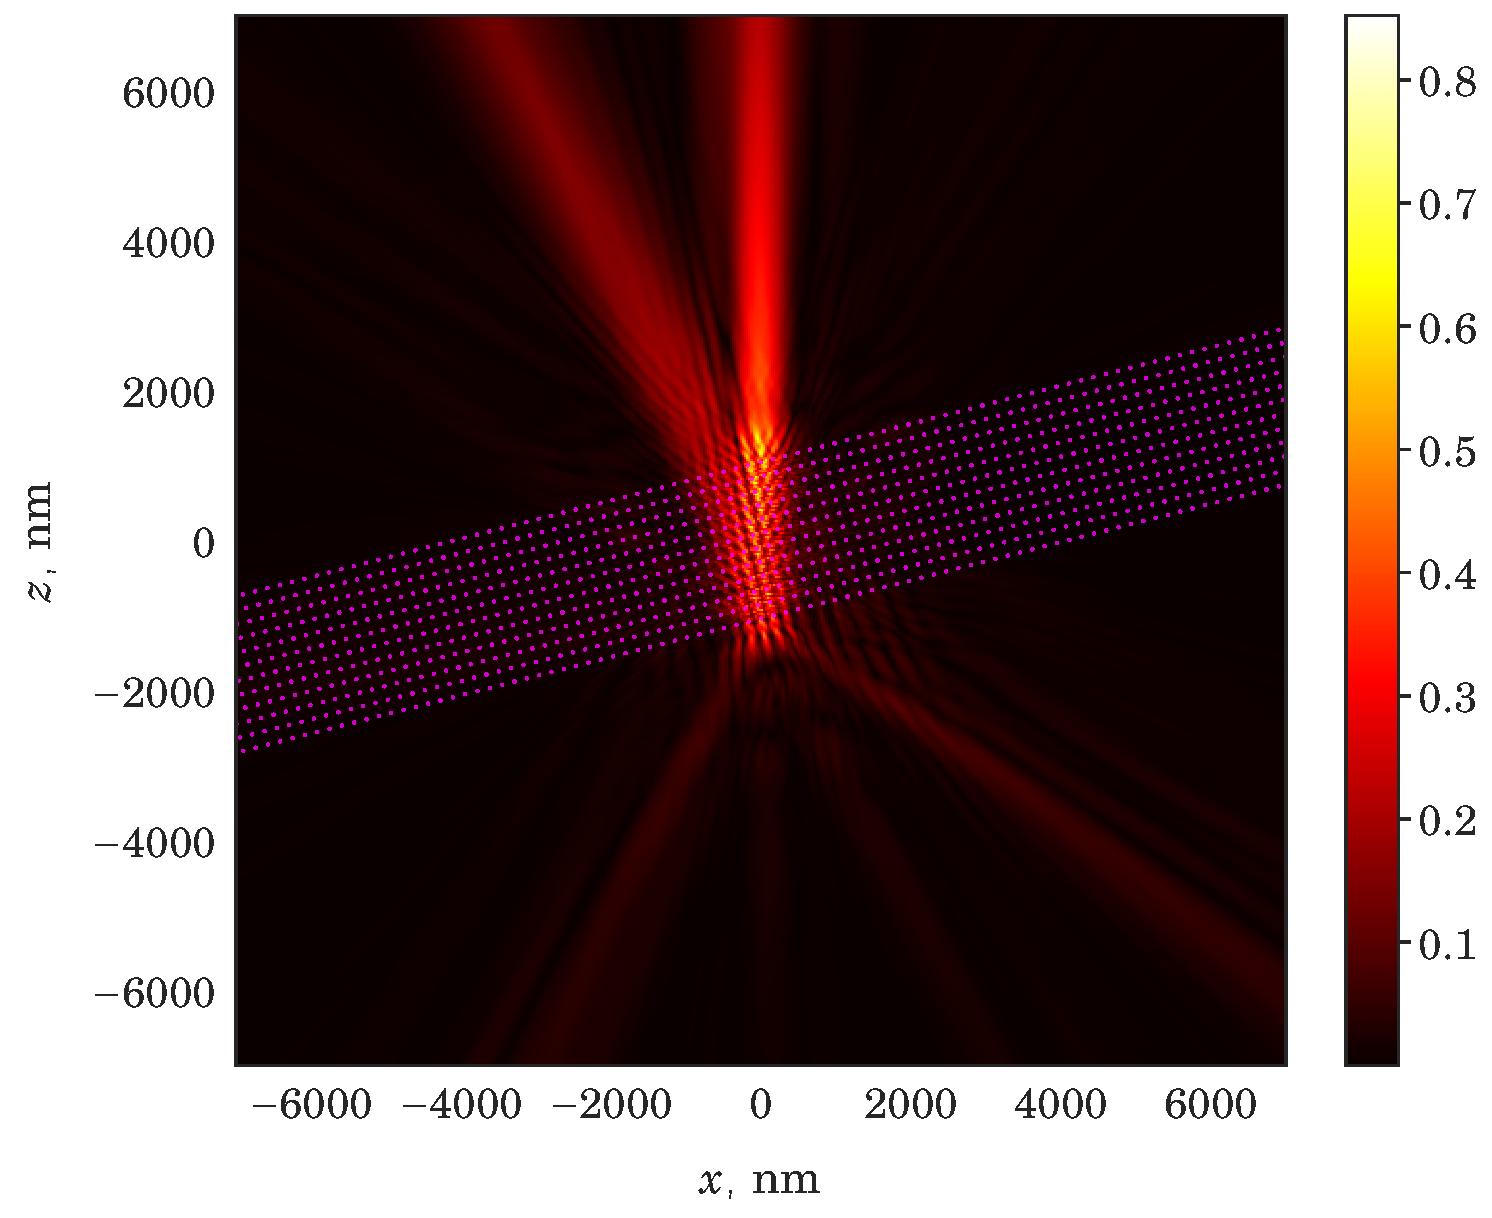
\includegraphics[width=0.9\columnwidth]{../components/img/celes/TE_14.324deg_check.pdf}}
	\caption{Scattered electric field normalized by the incident beam amplitude, the glancing angle $\theta = \arcsin\frac{1}{4}$, the grating period $d = 2\lambda_{10}$.}
	\label{14.324deg:image}
\end{figure}

\begin{figure}[htbp]
	\centerline{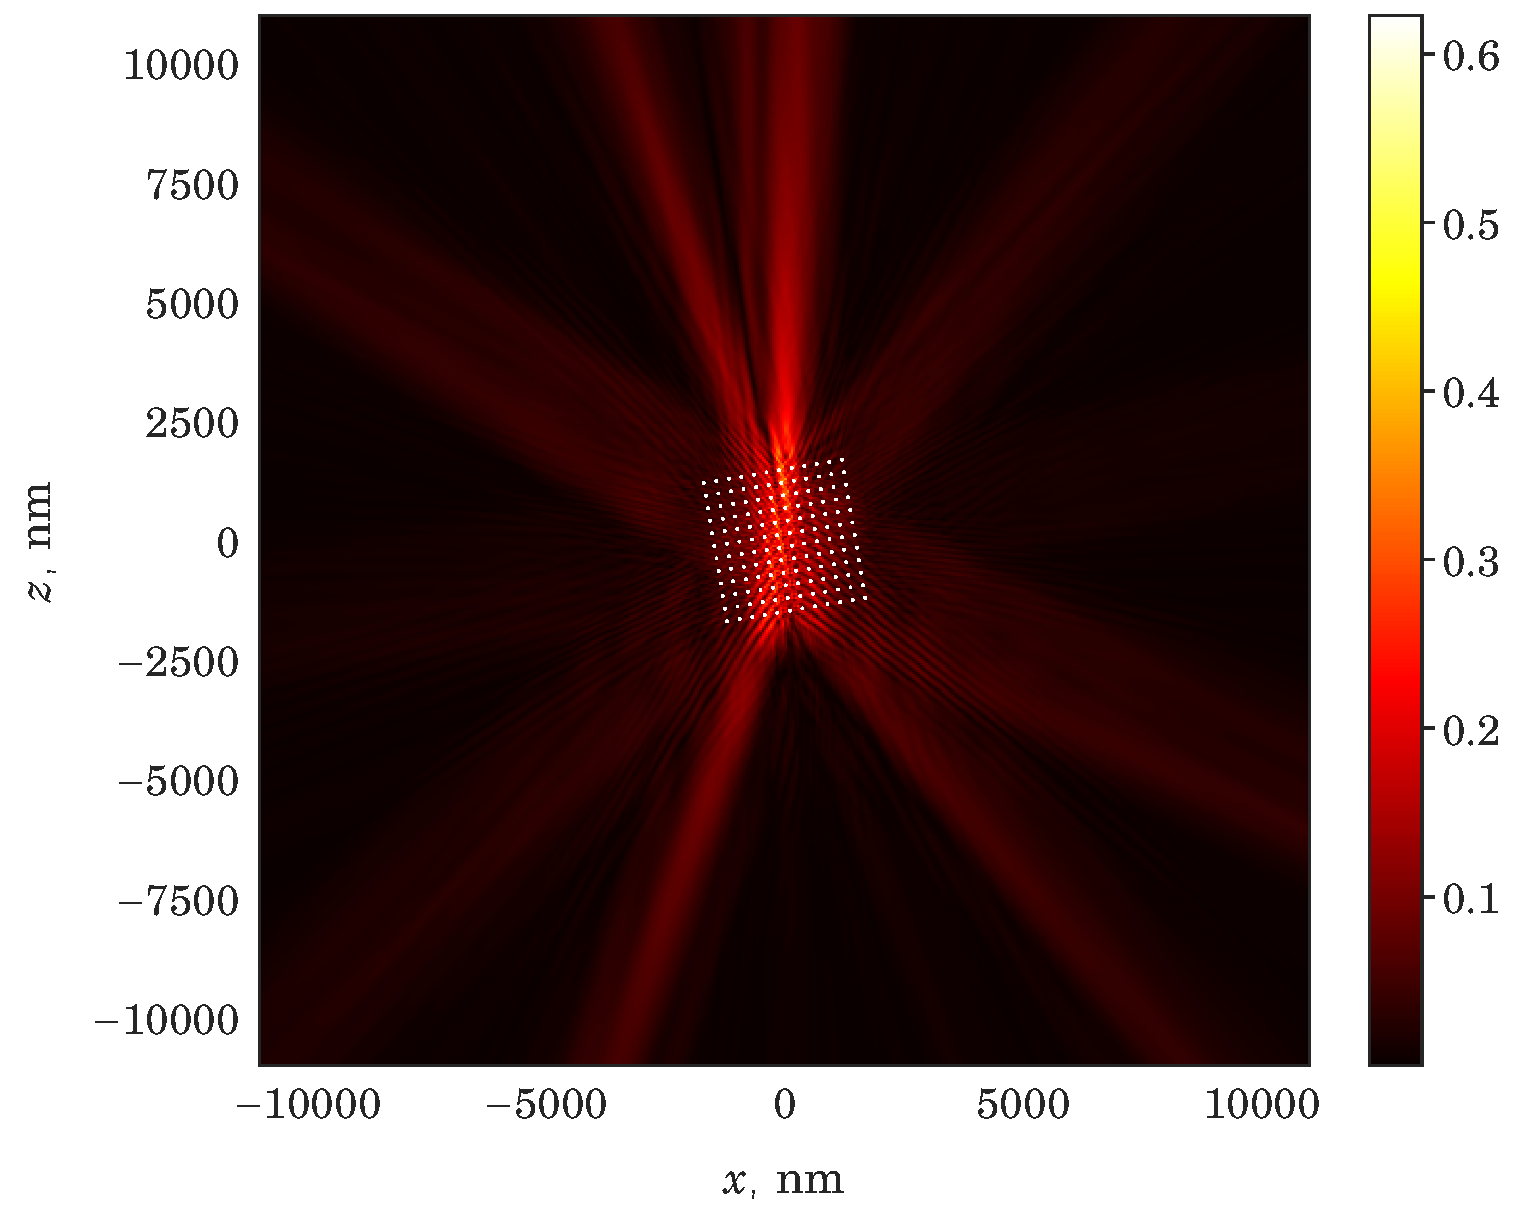
\includegraphics[width=0.9\columnwidth]{../components/img/celes/TE_9.594deg_check_3lambda.pdf}}
	\caption{Scattered electric field normalized by the incident beam amplitude, the glancing angle $\theta = \arcsin\frac{1}{6}$, the grating period $d = 3\lambda_{10}$.}
	\label{9.594deg:image}
\end{figure}

% Figure Labels: Use 8 point Times New Roman for Figure labels. Use words 
% rather than symbols or abbreviations when writing Figure axis labels to 
% avoid confusing the reader. As an example, write the quantity 
% ``Magnetization'', or ``Magnetization, M'', not just ``M''. If including 
% units in the label, present them within parentheses. Do not label axes only 
% with units. In the example, write ``Magnetization (A/m)'' or ``Magnetization 
% \{A[m(1)]\}'', not just ``A/m''. Do not label axes with a ratio of 
% quantities and units. For example, write ``Temperature (K)'', not 
% ``Temperature/K''.

\section*{Conclusion}

The results show the correspondence of the Bragg-Wolfe diffraction theory for planar and spatial gratings, the ability to control high harmonics of laser radiation (XUV range) using an ionized cluster gas.

% \begin{thebibliography}{00}
% \bibitem{b1} G. Eason, B. Noble, and I. N. Sneddon, ``On certain integrals of Lipschitz-Hankel type involving products of Bessel functions,'' Phil. Trans. Roy. Soc. London, vol. A247, pp. 529--551, April 1955.
% \bibitem{b2} J. Clerk Maxwell, A Treatise on Electricity and Magnetism, 3rd ed., vol. 2. Oxford: Clarendon, 1892, pp.68--73.
% \bibitem{b3} I. S. Jacobs and C. P. Bean, ``Fine particles, thin films and exchange anisotropy,'' in Magnetism, vol. III, G. T. Rado and H. Suhl, Eds. New York: Academic, 1963, pp. 271--350.
% \bibitem{b4} K. Elissa, ``Title of paper if known,'' unpublished.
% \bibitem{b5} R. Nicole, ``Title of paper with only first word capitalized,'' J. Name Stand. Abbrev., in press.
% \bibitem{b6} Y. Yorozu, M. Hirano, K. Oka, and Y. Tagawa, ``Electron spectroscopy studies on magneto-optical media and plastic substrate interface,'' IEEE Transl. J. Magn. Japan, vol. 2, pp. 740--741, August 1987 [Digests 9th Annual Conf. Magnetics Japan, p. 301, 1982].
% \bibitem{b7} M. Young, The Technical Writer's Handbook. Mill Valley, CA: University Science, 1989.

% \bibitem{boren_huffman} C. Bohren D. and Huffman ``Absorption and scattering of light by small particles''. Moscow, Mir, 1986
% \end{thebibliography}

\selectbiblanguage{english}
\bibliographystyle{ieeetr}
\bibliography{../components/bibliography.bib}

\end{document}
